

%% AAPT Physics Olympiad F=ma Questions
%%----------------------------------------


%% this section contains 40 problems


%% PhysicsOlympiad 2015
%%----------------------------------------
\element{aapt}{ %% Olympiad-A1
\begin{question}{Olympiad-2015-Q02}
    A car travels directly north on a straight highway at a constant speed of \SI{80}{\kilo\meter\per\hour} for a distance of \SI{25}{\kilo\meter}.
    The car then continues directly north at a constant speed of \SI{50}{\kilo\meter\per\hour} for a distance of \SI{75}{\kilo\meter}.
    The average speed of the car for the entire journey is closest to:
    \begin{multicols}{2}
    \begin{choices}
      \correctchoice{\SI{55.2}{\kilo\meter\per\hour}}
        \wrongchoice{\SI{57.5}{\kilo\meter\per\hour}}
        \wrongchoice{\SI{65}{\kilo\meter\per\hour}}
        \wrongchoice{\SI{69.6}{\kilo\meter\per\hour}}
        \wrongchoice{\SI{72.5}{\kilo\meter\per\hour}}
    \end{choices}
    \end{multicols}
\end{question}
}


%% PhysicsOlympiad 2014
%%----------------------------------------


%% PhysicsOlympiad 2013
%%----------------------------------------
\element{aapt}{ %% Olympiad-A1
\begin{question}{Olympiad-2013-Q01}
    An observer stands on the side of the front of a stationary train.
    When the train starts moving with constant acceleration,
        it takes \SI{5}{\second} for the first car to pass the observer.
    How long will it take for the 10th car to pass?
    \begin{multicols}{3}
    \begin{choices}
        %% T_10 - T_9 = \sqrt{10*5^2} - \sqrt{9*5^2}
        \wrongchoice{\SI{1.07}{\second}}
        \wrongchoice{\SI{0.98}{\second}}
        \wrongchoice{\SI{0.91}{\second}}
        \wrongchoice{\SI{0.86}{\second}}
      \correctchoice{\SI{0.81}{\second}}
    \end{choices}
    \end{multicols}
\end{question}
}


%% PhysicsOlympiad 2012
%%----------------------------------------
\element{aapt}{ %% Olympiad-A1
\begin{question}{Olympiad-2012-Q01}
    Consider a dripping faucet, where the faucet is \SI{10}{\centi\meter} above the sink.
    The time between drops is such that when one drop hits the sink,
        one is in the air and another is about to drop.
    At what height above the sink will the drop in the air be right as a drop hits the sink?
    \begin{choices}
        \wrongchoice{Between \SI{0}{\centi\meter} and \SI{2}{\centi\meter}}
        \wrongchoice{Between \SI{2}{\centi\meter} and \SI{4}{\centi\meter}}
        \wrongchoice{Between \SI{4}{\centi\meter} and \SI{6}{\centi\meter}}
      \correctchoice{Between \SI{6}{\centi\meter} and \SI{8}{\centi\meter}}
        \wrongchoice{Between \SI{8}{\centi\meter} and \SI{10}{\centi\meter}}
    \end{choices}
\end{question}
}


%% PhysicsOlympiad 2011
%%----------------------------------------
\element{aapt}{ %% Olympiad-A1
\begin{question}{Olympiad-2011-Q01}
    A cyclist travels at a constant speed of \SI{22.0}{\kilo\meter\per\hour}
        except for a \SI{20}{\minute} stop.
    The cyclist's average speed was \SI{17.5}{\kilo\meter\per\hour}.
    How far did the cyclist travel?
    \begin{multicols}{2}
    \begin{choices}
        %% d = v \frac{ \bar{v} T }{ v - \bar{v} }
      \correctchoice{\SI{28.5}{\kilo\meter}}
        \wrongchoice{\SI{30.3}{\kilo\meter}}
        \wrongchoice{\SI{31.2}{\kilo\meter}}
        \wrongchoice{\SI{36.5}{\kilo\meter}}
        \wrongchoice{\SI{38.9}{\kilo\meter}}
    \end{choices}
    \end{multicols}
\end{question}
}
\newcommand{\myOlympiaGraphElevenQTwo}{
\begin{tikzpicture}
\begin{groupplot}[
        group style={
            group size=1 by 3,
            x descriptions at=edge bottom,
            y descriptions at=edge left,
        },
        axis y line=left,
        axis x line=bottom,
        axis line style={->},
        xlabel={time},
        ylabel={velocity},
        xtick={0,2,4,6,8,10},
        ytick={-2,0,2,4},
        y unit=\si{\meter\per\second},
        xmin=0,xmax=10.2,
        ymin=-3,ymax=4.2,
        grid=major,
        width=0.90\columnwidth,
        height=0.45\columnwidth,
    ]
    \nextgroupplot[
        title={Object I},
        line width=1pt,
    ] \addplot[domain=0:4] {x};
      \addplot[domain=4:10] {8-x};
    \nextgroupplot[
        title={Object II},
        line width=1pt,
    ] \addplot[domain=0:9] {2};
      \addplot[domain=9:10] {20-2*x};
    \nextgroupplot[
        title={Object III},
        line width=1pt,
        x unit=\si{\second},
    ] \addplot[domain=0:6] {x/3};
      \addplot[domain=6:10] {2};
\end{groupplot}
\end{tikzpicture}
}

\element{aapt}{ %% Olympiad-A1
\begin{question}{Olympiad-2011-Q02}
    The three graphs below show the velocity of three objects as a function of time.
    Each object is moving only in one dimension.
    \begin{center}
        \myOlympiaGraphElevenQTwo
    \end{center}
    Rank the \emph{magnitudes} of the average acceleration during the ten second interval.
    %% I: -2 m/s^2, II: -2 m/s^2, III: 2 m/s^2
    \begin{multicols}{2}
    \begin{choices}
        \wrongchoice{$I>II>III$}
        \wrongchoice{$II>I>III$}
        \wrongchoice{$III>II>I$}
        \wrongchoice{$I>II=III$}
      \correctchoice{$I=II=III$}
    \end{choices}
    \end{multicols}
\end{question}
}

\element{aapt}{ %% Olympiad-A1
\begin{question}{Olympiad-2011-Q03}
    The three graphs below show the velocity of three objects as a function of time.
    Each object is moving only in one dimension.
    \begin{center}
        \myOlympiaGraphElevenQTwo
    \end{center}
    Rank the \emph{magnitudes} of the maximum velocity during the ten second interval.
    %% I: 4 m/s, II: 2 m/s, III: 2 m/s
    \begin{multicols}{2}
    \begin{choices}
        \wrongchoice{$I>II>III$}
        \wrongchoice{$II>I>III$}
        \wrongchoice{$III>II>I$}
      \correctchoice{$I>II=III$}
        \wrongchoice{$I=II=III$}
    \end{choices}
    \end{multicols}
\end{question}
}

\element{aapt}{ %% Olympiad-A1
\begin{question}{Olympiad-2011-Q04}
    The three graphs below show the velocity of three objects as a function of time.
    Each object is moving only in one dimension.
    \begin{center}
        \myOlympiaGraphElevenQTwo
    \end{center}
    Rank the \emph{magnitudes} of the \emph{distance} traveled during the ten second interval.
    \begin{multicols}{2}
    \begin{choices}
        %% I: 18m, II: 19m, III: 14m
        \wrongchoice{$I>II>III$}
      \correctchoice{$II>I>III$}
        \wrongchoice{$III>II>I$}
        \wrongchoice{$I>II=III$}
        \wrongchoice{$I=II=III$}
    \end{choices}
    \end{multicols}
\end{question}
}


%% PhysicsOlympiad 2010
%%----------------------------------------
\newcommand{\olympiadTwentyTenQOne}{
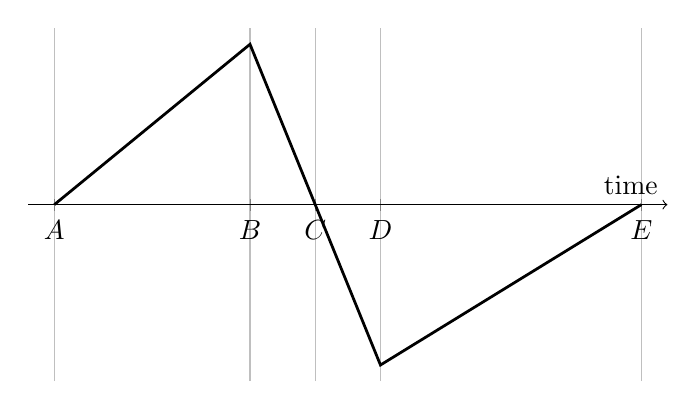
\begin{tikzpicture}
    \begin{axis}[
        clip=false,
        axis y line=none,
        axis x line=middle,
        axis line style={->},
        xlabel={time},
        xtick={0,3,4,5,9},
        xticklabels={$A$, $B$, $C$, $D$, $E$},
        ylabel=\empty,
        ytick={-4,-2,0,2,4},
        grid=major,
        ymin=-4.4,ymax=4.4,
        xmin=-0.4,xmax=9.4,
        width=0.8\columnwidth,
        height=0.5\columnwidth,
    ]
    \addplot[line width=1pt,mark=\empty] coordinates {(0,0) (3,4) (5,-4) (9,0) };
    \end{axis}
\end{tikzpicture}
}

\element{aapt}{ %% Olympiad-A1
\begin{question}{Olympiad-2010-Q01}
    The figure below represents the motion of a squirrel as it
        runs in a straight-line along a telephone wire.
    The letters $A$ through $E$ refer to the indicated times.
    \begin{center}
        \olympiadTwentyTenQOne
    \end{center}
    If the graph is a graph of Position vs. Time,
        then the squirrel has the greatest speed at what times(s)
        or during what time interval(s)?
    \begin{multicols}{2}
    \begin{choices}
        \wrongchoice{from $A$ to $B$}
        \wrongchoice{from $B$ to $C$ only}
      \correctchoice{from $B$ to $D$}
        \wrongchoice{from $C$ to $D$ only}
        \wrongchoice{from $D$ to $E$}
    \end{choices}
    \end{multicols}
\end{question}
}

\element{aapt}{ %% Olympiad-A1
\begin{question}{Olympiad-2010-Q02}
    The figure below represents the motion of a squirrel as it
        runs in a straight-line along a telephone wire.
    The letters $A$ through $E$ refer to the indicated times.
    \begin{center}
        \olympiadTwentyTenQOne
    \end{center}
    If the graph is a graph of Velocity vs. Time,
        then the squirrel has the greatest speed at what times(s)
        or during what time interval(s)?
    \begin{multicols}{2}
    \begin{choices}
        \wrongchoice{at $B$}
        \wrongchoice{at $C$}
        \wrongchoice{at $D$}
      \correctchoice{at both $B$ and $D$}
        \wrongchoice{From $C$ to $D$}
    \end{choices}
    \end{multicols}
\end{question}
}

\element{aapt}{ %% Olympiad-A1
\begin{question}{Olympiad-2010-Q03}
    The figure below represents the motion of a squirrel as it
        runs in a straight-line along a telephone wire.
    The letters $A$ through $E$ refer to the indicated times.
    \begin{center}
        \olympiadTwentyTenQOne
    \end{center}
    If the graph is a graph of Acceleration vs. Time,
        then the squirrel has the greatest speed at what times(s)
        or during what time interval(s)?
    \begin{choices}
        \wrongchoice{at $B$}
      \correctchoice{at $C$}
        \wrongchoice{at $D$}
        \wrongchoice{at both $B$ and $D$}
        \wrongchoice{From $C$ to $D$}
    \end{choices}
\end{question}
}


%% PhysicsOlympiad 2009
%%----------------------------------------
\element{aapt}{ %% Olympiad-A1
\begin{question}{Olympiad-2009-Q07}
    A bird is flying in a straight line initially at \SI{10}{\meter\per\second}.
    It uniformly increases its speed to \SI{15}{\meter\per\second}
        while covering a distance of \SI{25}{\meter}.
    What is the magnitude of the acceleration of the bird?
    \begin{multicols}{2}
    \begin{choices}
        \wrongchoice{\SI{5.0}{\meter\per\second\squared}}
      \correctchoice{\SI{2.5}{\meter\per\second\squared}}
        \wrongchoice{\SI{2.0}{\meter\per\second\squared}}
        \wrongchoice{\SI{0.5}{\meter\per\second\squared}}
        \wrongchoice{\SI{0.2}{\meter\per\second\squared}}
    \end{choices}
    \end{multicols}
\end{question}
}


%% PhysicsOlympiad 2008
%%----------------------------------------
\element{aapt}{ %% Olympiad-A1
\begin{question}{Olympiad-2008-Q01}
    A bird flying in a straight line, initially at \SI{10}{\meter\per\second},
        uniformly increases its speed to \SI{18}{\meter\per\second}
        while covering a distance of \SI{40}{\meter}.
    What is the magnitude of the acceleration of the bird?
    \begin{multicols}{2}
    \begin{choices}
        \wrongchoice{\SI{0.1}{\meter\per\second\squared}}
        \wrongchoice{\SI{0.2}{\meter\per\second\squared}}
        \wrongchoice{\SI{2.0}{\meter\per\second\squared}}
      \correctchoice{\SI{2.8}{\meter\per\second\squared}}
        \wrongchoice{\SI{5.6}{\meter\per\second\squared}}
    \end{choices}
    \end{multicols}
\end{question}
}

\element{aapt}{ %% Olympiad-A1
\begin{question}{Olympiad-2008-Q02}
    A cockroach is crawling along the walls inside a cubical room that
        has an edge length of \SI{3}{\meter}.
    If the cockroach starts from the back lower left hand corner of the
        cube and finishes at the front upper right hand corner,
        what is the magnitude of the displacement of the cockroach?
    \begin{multicols}{2}
    \begin{choices}
        \wrongchoice{\SI[parse-numbers=false]{3\sqrt{2}}{\meter}}
        \wrongchoice{\SI[parse-numbers=false]{3\sqrt[3]{2}}{\meter}}
      \correctchoice{\SI[parse-numbers=false]{3\sqrt{3}}{\meter}}
        \wrongchoice{\SI[parse-numbers=false]{3}{\meter}}
        \wrongchoice{\SI[parse-numbers=false]{9}{\meter}}
    \end{choices}
    \end{multicols}
\end{question}
}

\newcommand{\myOlympiadEightQzeroFour}{
\begin{tikzpicture}
    \begin{axis}[
        axis y line=left,
        axis x line=middle,
        axis line style={->},
        xlabel={time},
        x unit=\si{\second},
        xtick={0,1,2,3},
        minor x tick num=1,
        ylabel={velocity},
        y unit=\si{\meter\per\second},
        ytick={-2,0,2,4},
        minor x tick num=1,
        grid=major,
        xmin=0,xmax=3.3,
        ymin=-2.5,ymax=4.5,
        width=0.8\columnwidth,
        height=0.5\columnwidth,
    ]
    \addplot[line width=1pt,mark=\empty] plot coordinates { (0,2) (1,4) (1.5,4) (3,-2) };
    \end{axis}
\end{tikzpicture}
}

\element{aapt}{ %% Olympiad-A1
\begin{question}{Olympiad-2008-Q04}
    Shown below is the velocity vs. time graph for a toy car moving along a straight line.
    \begin{center}
        \myOlympiadEightQzeroFour
    \end{center}
    What is the maximum displacement from start for the toy car?
    \begin{multicols}{3}
    \begin{choices}
        \wrongchoice{\SI{3}{\meter}}
        \wrongchoice{\SI{5}{\meter}}
        \wrongchoice{\SI{6.5}{\meter}}
      \correctchoice{\SI{7}{\meter}}
        \wrongchoice{\SI{7.5}{\meter}}
    \end{choices}
    \end{multicols}
\end{question}
}

\element{aapt}{ %% Olympiad-A1
\begin{question}{Olympiad-2008-Q05}
    Shown below is the velocity vs. time graph for a toy car moving along a straight line.
    \begin{center}
        \myOlympiadEightQzeroFour
    \end{center}
    Which of the following acceleration vs. time graphs most closely
        represents the acceleration of the toy car
    \begin{choices}
        \AMCboxDimensions{down=-1.5em}
        \wrongchoice{
            \begin{tikzpicture}
                \begin{axis}[
                    axis y line=left,
                    axis x line=middle,
                    axis line style={->},
                    xlabel={time},
                    x unit=\si{\second},
                    xtick={0,1,2,3},
                    %ylabel={$a$},
                    %y unit=\si{\meter\per\second\squared},
                    ytick={-2,0,2},
                    grid=major,
                    xmin=0,xmax=3.2,
                    ymin=-2.2,ymax=2.2,
                    width=0.8\columnwidth,
                    height=0.4\columnwidth,
                ]
                \addplot[line width=1pt,mark=\empty] plot coordinates {(0,2) (1,2) (1,0) (1.5,0) (1.5,1) (3,1)};
                \end{axis}
            \end{tikzpicture}
        }
        \wrongchoice{
            \begin{tikzpicture}
                \begin{axis}[
                    axis y line=left,
                    axis x line=middle,
                    axis line style={->},
                    xlabel={time},
                    x unit=\si{\second},
                    xtick={0,1,2,3},
                    %ylabel={$a$},
                    %y unit=\si{\meter\per\second\squared},
                    ytick={-2,0,2},
                    grid=major,
                    xmin=0,xmax=3.2,
                    ymin=-2.2,ymax=2.2,
                    width=0.8\columnwidth,
                    height=0.4\columnwidth,
                ]
                \addplot[line width=1pt,mark=\empty] plot coordinates {(0,2) (1,2) (1,0) (1.5,0) (1.5,-1) (3,-1)};
                \end{axis}
            \end{tikzpicture}
        }
        %% ANS is C
        \correctchoice{
            \begin{tikzpicture}
                \begin{axis}[
                    axis y line=left,
                    axis x line=middle,
                    axis line style={->},
                    xlabel={time},
                    x unit=\si{\second},
                    xtick={0,1,2,3},
                    %ylabel={$a$},
                    %y unit=\si{\meter\per\second\squared},
                    ytick={-2,0,2},
                    grid=major,
                    xmin=0,xmax=3.2,
                    ymin=-2.2,ymax=2.2,
                    width=0.8\columnwidth,
                    height=0.4\columnwidth,
                ]
                \addplot[line width=1pt,mark=\empty] plot coordinates {(0,1) (1,1) (1,0) (1.5,0) (1.5,-2) (3,-2)};
                \end{axis}
            \end{tikzpicture}
        }
        \wrongchoice{
            \begin{tikzpicture}
                \begin{axis}[
                    axis y line=left,
                    axis x line=middle,
                    axis line style={->},
                    xlabel={time},
                    x unit=\si{\second},
                    xtick={0,1,2,3},
                    %ylabel={$a$},
                    %y unit=\si{\meter\per\second\squared},
                    ytick={-2,0,2},
                    grid=major,
                    xmin=0,xmax=3.2,
                    ymin=-2.2,ymax=2.2,
                    width=0.8\columnwidth,
                    height=0.4\columnwidth,
                ]
                \addplot[line width=1pt,mark=\empty] plot coordinates {(0,1) (1,1) (1,0) (1.5,0) (1.5,-2) (2.5,-2) (2.5,2) (3,2)};
                \end{axis}
            \end{tikzpicture}
        }
        \wrongchoice{
            \begin{tikzpicture}
                \begin{axis}[
                    axis y line=left,
                    axis x line=middle,
                    axis line style={->},
                    xlabel={time},
                    x unit=\si{\second},
                    xtick={0,1,2,3},
                    %ylabel={$a$},
                    %y unit=\si{\meter\per\second\squared},
                    ytick={-2,0,2},
                    grid=major,
                    xmin=0,xmax=3.2,
                    ymin=-2.2,ymax=2.2,
                    width=0.8\columnwidth,
                    height=0.4\columnwidth,
                ]
                \addplot[line width=1pt,mark=\empty] plot coordinates {(0,2) (1,2) (1,1) (1.5,1) (1.5,-1) (2.5,-1) (2.5,1) (3,1)};
                \end{axis}
            \end{tikzpicture}
        }
    \end{choices}
\end{question}
}

\element{aapt}{ %% Olympiad-A1
\begin{question}{Olympiad-2008-Q24}
    A ball is launched upward from the ground at an initial vertical speed
        of $v_0$ and begins bouncing vertically.
    Every time it rebounds,
        it loses a proportion of the magnitude of its velocity due to the
        inelastic nature of the collision,
        such that if the speed just before hitting the ground on a bounce is $v$,
        then the speed just after the bounce is $rv$, where $r<1$ is a constant.
    Calculate the total length of time that the ball remains bouncing,
        assuming that any time associated with the actual contact
        of the ball with the ground is negligible.
    \begin{multicols}{2}
    \begin{choices}
      \correctchoice{$\dfrac{2v_0}{g}\dfrac{1}{1-r}$}
        \wrongchoice{$\dfrac{v_0}{g}\dfrac{r}{1-r}$}
        \wrongchoice{$\dfrac{2v_0}{g}\dfrac{1-r}{r}$}
        \wrongchoice{$\dfrac{2v_0}{g}\dfrac{1}{1-r^2}$}
        \wrongchoice{$\dfrac{2v_0}{g}\dfrac{1}{1+(1-r)^2}$}
    \end{choices}
    \end{multicols}
\end{question}
}


%% PhysicsOlympiad 2007
%%----------------------------------------
\element{aapt}{ %% Olympiad-A1
\begin{question}{Olympiad-2007-Q01}
    An object moves in two dimensions according to
    \begin{equation*}
        \vec{r}\left(t\right) = \left( 4.0 t^2-9.0\right) \hat{\imath} +
                                \left( 2.0 t - 5.0\right) \hat{\jmath},
    \end{equation*}
    where $r$ is in meters and $g$ in seconds.
    When does the object cross the $x$-axis?
    \begin{multicols}{3}
    \begin{choices}
        \wrongchoice{\SI{0.0}{\second}}
        \wrongchoice{\SI{0.4}{\second}}
        \wrongchoice{\SI{0.6}{\second}}
        \wrongchoice{\SI{1.5}{\second}}
      \correctchoice{\SI{2.5}{\second}}
    \end{choices}
    \end{multicols}
\end{question}
}

\element{aapt}{ %% Olympiad-A1
\begin{question}{Olympiad-2007-Q03}
    The coordinate of an object is given as a function of time by
        $x = 8 t - 3 t^2$, where $x$ is in meters and $t$ is in seconds.
    Its average velocity over the interval from $t = \SIrange{1}{2}{\second}$ is
    \begin{multicols}{3}
    \begin{choices}
        \wrongchoice{\SI{-2}{\meter\per\second}}
      \correctchoice{\SI{-1}{\meter\per\second}}
        \wrongchoice{\SI{-0.5}{\meter\per\second}}
        \wrongchoice{\SI{0.5}{\meter\per\second}}
        \wrongchoice{\SI{1}{\meter\per\second}}
    \end{choices}
    \end{multicols}
\end{question}
}

\element{aapt}{ %% Olympiad-A1
\begin{question}{Olympiad-2007-Q04}
    An object is released from rest and falls a distance
        $h$ during the first second of time.
    How far will it fall during the next second of time?
    \begin{multicols}{3}
    \begin{choices}
        \wrongchoice{$h$}
        \wrongchoice{$2h$}
      \correctchoice{$3h$}
        \wrongchoice{$4h$}
        \wrongchoice{$h^2$}
    \end{choices}
    \end{multicols}
\end{question}
}

\element{aapt}{ %% Olympiad-A1
\begin{question}{Olympiad-2007-Q06}
    At time $t = 0$ a drag racer starts from rest at the origin
        and moves along a straight line with velocity given by $v=5t^2$,
        where $v$ is in \si{\meter\per\second} and $t$ is in \si{\second}.
    The expression for the displacement of the car from $t=0$ to time $t$ is
    \begin{multicols}{3}
    \begin{choices}
        \wrongchoice{$5t^3$}
      \correctchoice{$\dfrac{5t^3}{3}$}
        \wrongchoice{$10t$}
        \wrongchoice{$15t^2$}
        \wrongchoice{$\dfrac{5t}{2}$}
    \end{choices}
    \end{multicols}
\end{question}
}


%% PhysicsOlympiad 2004
%%----------------------------------------
\element{aapt}{ %% Olymmpiad-A1
\begin{question}{Olympiad-2004-Q01}
    A stone is thrown straight downward with a speed of \SI{20}{\meter\per\second} from the top of a tall building.
    If the stone strikes the ground \SI{3.0}{\second} later,
        how tall is the building?
    \begin{multicols}{3}
    \begin{choices}
        \wrongchoice{\SI{45}{\meter}}
        \wrongchoice{\SI{60}{\meter}}
        \wrongchoice{\SI{90}{\meter}}
      \correctchoice{\SI{105}{\meter}}
        \wrongchoice{\SI{120}{\meter}}
    \end{choices}
    \end{multicols}
\end{question}
}

\element{aapt}{ %% Olympiad-A1
\begin{question}{Olympiad-2004-Q02}
    A coyote can run at a speed of \SI{20}{\meter\per\second} while a prairie dog can manage only \SI{5.5}{\meter\per\second}.
    If the prairie dog is \SI{45}{\meter} in front of a coyote,
        what is the maximum time it has to reach its hole without being caught?
    \begin{multicols}{3}
    \begin{choices}
        \wrongchoice{\SI{2.3}{\second}}
      \correctchoice{\SI{3.1}{\second}}
        \wrongchoice{\SI{5.4}{\second}}
        \wrongchoice{\SI{5.9}{\second}}
        \wrongchoice{\SI{8.2}{\second}}
    \end{choices}
    \end{multicols}
\end{question}
}

\element{aapt}{ %% Olympiad-A1
\begin{question}{Olympiad-2004-Q03}
    A model rocket accelerates upwards at \SI{50}{\meter\per\second\squared} for \SI{2.0}{\second} before its engine burns out.
    The rocket then coasts upward.
    What is the maximum height that the rocket reaches?
    You may assume air resistance is negligible.
    \begin{multicols}{3}
    \begin{choices}
        \wrongchoice{\SI{100}{\meter}}
        \wrongchoice{\SI{510}{\meter}}
      \correctchoice{\SI{610}{\meter}}
        \wrongchoice{\SI{1020}{\meter}}
        \wrongchoice{\SI{1220}{\meter}}
    \end{choices}
    \end{multicols}
\end{question}
}

\element{aapt}{ %% Olympiad-A1
\begin{question}{Olympiad-2004-Q13}
    A baseball is thrown vertically into the air with a velocity $v$,
        and reaches a maximum height $h$.
    At what height was the baseball moving with one-half its original velocity?
    Assume air resistance is negligible.
    \begin{multicols}{3}
    \begin{choices}
        \wrongchoice{$\dfrac{h}{4}$}
        \wrongchoice{$\dfrac{h}{3}$}
        \wrongchoice{$\dfrac{h}{2}$}
        \wrongchoice{$\dfrac{2h}{3}$}
      \correctchoice{$\dfrac{3h}{4}$}
    \end{choices}
    \end{multicols}
\end{question}
}

\newcommand{\OlympiadTwentyZeroFourQEighteen}{
\begin{tikzpicture}
    \node at (1,5) {Top};
    %% Ground
    \node[anchor=north,fill,pattern=north east lines,minimum width=2.4cm, minimum height=0.1cm] at (0.8,0) {};
    \draw (0,0) -- (2,0);
    %% Building
    \draw (-0.4cm,0) rectangle (0,5cm);
    \node[anchor=center,fill,pattern=north east lines,minimum width=0.4cm, minimum height=5cm] at (-0.2,2.5) {};
    %% ball A
    \node[circle,fill] (A) at (1,2) {};
    \node[anchor=west] at (A.east) {Ball $A$};
    %% ball B
    \node[circle,fill] (B) at (1,4) {};
    \node[anchor=west] at (B.east) {Ball $B$};
\end{tikzpicture}
}

\element{aapt}{ %% Olympiad-A1
\begin{question}{Olympiad-2004-Q18}
    Two identical bowling balls $A$ and $B$ are each dropped from rest from the top of a tall tower as shown at the right.
    Ball $A$ is dropped \SI{1.0}{\second} before ball $B$ is dropped but both balls fall for some time before ball $A$ strikes the ground.
    \begin{center}
        \OlympiadTwentyZeroFourQEighteen
    \end{center}
    Air resistance can be considered negligible during the fall.
    %% start question
    At the moment ball $B$ is released:
    \begin{choices}
        \wrongchoice{ball $A$ has fallen about \SI{10}{\meter}}
      \correctchoice{ball $A$ is traveling at about \SI{10}{\meter\per\second}}
        \wrongchoice{its acceleration is about \SI{10}{\meter\per\second\squared} less than ball $A$}
        \wrongchoice{ball $A$ has more mechanical energy than ball $B$}
        \wrongchoice{ball $B$ has more mechanical energy than ball $A$}
    \end{choices}
\end{question}
}

\element{aapt}{ %% Olympiad-A1
\begin{question}{Olympiad-2004-Q19}
    Two identical bowling balls $A$ and $B$ are each dropped from rest from the top of a tall tower as shown at the right.
    Ball $A$ is dropped \SI{1.0}{\second} before ball $B$ is dropped but both balls fall for some time before ball $A$ strikes the ground.
    \begin{center}
        \OlympiadTwentyZeroFourQEighteen
    \end{center}
    Air resistance can be considered negligible during the fall.
    %% start question
    After ball $B$ is dropped but before ball $A$ strikes the ground,
    \begin{choices}
      \correctchoice{the distance between the two balls increases}
        \wrongchoice{the distance between the two balls decreases}
        \wrongchoice{the distance between the two balls remains constant}
        \wrongchoice{the velocity of ball $A$ increases with respect to ball $B$}
        \wrongchoice{the velocity of ball $A$ decreases with respect to ball $B$}
    \end{choices}
\end{question}
}


%% PhysicsOlympiad 2003
%%----------------------------------------



%% PhysicsOlympiad 2000
%%----------------------------------------
\newcommand{\aaptOlympiadZeroZeroQOne}{
\begin{tikzpicture}
    \begin{axis}[
        axis y line=left,
        axis x line=middle,
        axis line style={->},
        xlabel={time},
        x unit=\si{\second},
        xtick={0,2,4,6,8},
        minor x tick num=1,
        ylabel={acceleration},
        y unit=\si{\meter\per\second\squared},
        ytick={-4,-2,0,2,4},
        minor y tick num=1,
        grid=major,
        xmin=0,xmax=8,
        ymin=-4.5,ymax=4.5,
        width=0.8\columnwidth,
        height=0.5\columnwidth,
    ]
    \addplot[line width=1pt,no marks] plot coordinates { (0,0) (2,4) (6,-4) (8,0) };
    \end{axis}
\end{tikzpicture}
}

\element{aapt}{ %% Olympiad-A1
\begin{question}{olympiad-2000-q01}
    A car moves as described in the acceleration vs time graph below.
    \begin{center}
        \aaptOlympiadZeroZeroQOne
    \end{center}
    At what time would the car be moving with the greatest velocity?
    \begin{multicols}{3}
    \begin{choices}
        \wrongchoice{\SI{0}{\second}}
        \wrongchoice{\SI{2}{\second}}
      \correctchoice{\SI{4}{\second}}
        \wrongchoice{\SI{6}{\second}}
        \wrongchoice{\SI{8}{\second}}
    \end{choices}
    \end{multicols}
\end{question}
}

\element{aapt}{ %% Olympiad-A1
\begin{question}{olympiad-2000-q02}
    A car moves as described in the acceleration vs time graph below.
    \begin{center}
        \aaptOlympiadZeroZeroQOne
    \end{center}
    At what time would the car be farthest from its original starting position?
    \begin{multicols}{3}
    \begin{choices}
        \wrongchoice{\SI{0}{\second}}
        \wrongchoice{\SI{2}{\second}}
        \wrongchoice{\SI{4}{\second}}
        \wrongchoice{\SI{6}{\second}}
      \correctchoice{\SI{8}{\second}}
    \end{choices}
    \end{multicols}
\end{question}
}


%% PhysicsOlympiad 1999
%%----------------------------------------
\element{aapt}{ %% Olympiad-A1
\begin{question}{olympiad-1999-q01}
    A truck driver travels three-fourths the distance of his run at one velocity ($v$) and then completes his run at one half his original velocity ($1⁄2v$).
    What was the trucker's average speed for the trip?
    \begin{multicols}{3}
    \begin{choices}
        \wrongchoice{$0.85v$}
      \correctchoice{$0.80v$}
        \wrongchoice{$0.75v$}
        \wrongchoice{$0.70v$}
        \wrongchoice{$0.65v$}
    \end{choices}
    \end{multicols}
\end{question}
}


%% PhysicsOlympiad 1998
%%----------------------------------------
\element{aapt}{ %% Olympiad-A1
\begin{question}{olympiad-1998-q04}
    A child tosses a ball directly upward.
    Its total time in the air is $T$.
    Its maximum height is $H$.
    What is its height after it has been in the air a time $T/4$?
    Neglect air resistance.
    \begin{multicols}{3}
    \begin{choices}
        \wrongchoice{$\dfrac{1}{4} H$}
        \wrongchoice{$\dfrac{1}{3} H$}
        \wrongchoice{$\dfrac{1}{2} H$}
        \wrongchoice{$\dfrac{2}{3} H$}
      \correctchoice{$\dfrac{3}{4} H$}
    \end{choices}
    \end{multicols}
\end{question}
}

\element{aapt}{ %% Olympiad-A1
\begin{questionmult}{olympiad-1998-q05}
    A whiffle ball is tossed straight up,
        reaches a highest point, and falls back down.
    Air resistance is not negligible.
    Which of the following statements are true?
    \begin{choices}
      \correctchoice{The ball's speed is zero at the highest point.}
        \wrongchoice{The ball's acceleration is zero at the highest point.}
        \wrongchoice{The ball takes a longer time to travel up to the highest point than to fall back down.}
        %% A. I only B. II only C. I & II only D. I & III only E. I, II, & III
    \end{choices}
\end{questionmult}
}


%% PhysicsOlympiad 1997
%%----------------------------------------
\element{aapt}{ %% Olympiad-A1
\begin{question}{olympiad-1997-q01}
    Starting from rest at time $t=0$,
        a car moves in a straight line with an acceleration given by the accompanying graph.
    \begin{center}
    \begin{tikzpicture}
        \begin{axis}[
            axis y line=left,
            axis x line=bottom,
            axis line style={->},
            xlabel={time},
            x unit=\si{\second},
            xtick={0,2,4,6},
            minor x tick num=1,
            ylabel={acceleration},
            y unit=\si{\meter\per\second\squared},
            ytick={0,2,4,6},
            minor y tick num=1,
            grid=major,
            xmin=0,xmax=6.1,
            ymin=0,ymax=6.2,
            width=0.8\columnwidth,
            height=0.5\columnwidth,
        ]
        \addplot[line width=1.5pt,no marks] plot coordinates { (0,5) (5,0) (6,0) };
        \end{axis}
    \end{tikzpicture}
    \end{center}
    What is the speed of the car at $t=\SI{3}{\second}$?
    \begin{multicols}{3}
    \begin{choices}
        \wrongchoice{\SI{1.0}{\meter\per\second}}
        \wrongchoice{\SI{2.0}{\meter\per\second}}
        \wrongchoice{\SI{6.0}{\meter\per\second}}
      \correctchoice{\SI{10.5}{\meter\per\second}}
        \wrongchoice{\SI{12.5}{\meter\per\second}}
    \end{choices}
    \end{multicols}
\end{question}
}


%% PhysicsOlympiad 1996
%%----------------------------------------
\element{aapt}{ %% Olympiad-A1
\begin{question}{olympiad-1996-q01}
    An object is projected straight upward from ground level with a velocity of \SI{50}{\meter\per\second}.
    Ignoring air resistance,
        it will return to ground level in approximately:
    \begin{multicols}{3}
    \begin{choices}
        \wrongchoice{\SI{2.5}{\second}}
        \wrongchoice{\SI{5.0}{\second}}
        \wrongchoice{\SI{7.5}{\second}}
      \correctchoice{\SI{10}{\second}}
        \wrongchoice{\SI{15}{\second}}
    \end{choices}
    \end{multicols}
\end{question}
}

\element{aapt}{ %% Olympiad-A1
\begin{question}{olympiad-1996-q03}
    A ball is thrown downward with speed \SI{15}{\meter\per\second} from the roof of a \SI{30}{\meter} building.
    At the same instant a ball is thrown upward with speed \SI{15}{\meter\per\second} from ground level.
    Relative to ground level,
        the two balls pass each other at a height of:
    \begin{multicols}{3}
    \begin{choices}
        \wrongchoice{zero}
        \wrongchoice{\SI{5.0}{\meter}}
      \correctchoice{\SI{10}{\meter}}
        \wrongchoice{\SI{15}{\meter}}
        \wrongchoice{\SI{20}{\meter}}
    \end{choices}
    \end{multicols}
\end{question}
}


%% PhysicsOlympiad 1995
%%----------------------------------------
\element{aapt}{ %% Olympiad-A1
\begin{question}{olympiad-1995-q07}
    Car $A$ and car $B$ are both traveling down a straight highway at \SI{25}{\meter\per\second} (about \SI{56}{\mile\per\hour}).
    Car $A$ is only \SI{6.0}{\meter} behind car $B$.
    The driver of car $B$ brakes,
        slowing down with a constant acceleration of \SI{2.0}{\meter\per\second\squared}.
    After a time \SI{1.2}{\second},
        the driver of car $A$ begins to brake,
        also at \SI{2.0}{\meter\per\second\squared}.
    What is the relative velocity of the two cars when they collide?
    Hint: Both cars are still moving forward when they collide.
    \begin{multicols}{3}
    \begin{choices}
      \correctchoice{\SI{2.4}{\meter\per\second}}
        \wrongchoice{\SI{5.0}{\meter\per\second}}
        \wrongchoice{\SI{9.5}{\meter\per\second}}
        \wrongchoice{\SI{21}{\meter\per\second}}
        \wrongchoice{\SI{24}{\meter\per\second}}
    \end{choices}
    \end{multicols}
\end{question}
}

\element{aapt}{ %% Olympiad-A1
\begin{question}{olympiad-1995-q18}
    A firecracker exploding on the surface of a lake is heard as two sounds---a time interval $t$ apart---by the paddler of a nearby canoe.
    Sound travels with a speed $u$ in water and a speed $v$ in air.
    The distance from the exploding firecracker to the canoe is:
    \begin{multicols}{3}
    \begin{choices}
        \wrongchoice{$\dfrac{uvt}{u+v}$}
        \wrongchoice{$\dfrac{t\left(u+v\right)}{uv}$}
        \wrongchoice{$\dfrac{t\left(u-v\right)}{uv}$}
        \wrongchoice{$vt$}
      \correctchoice{$\dfrac{uvt}{u-v}$}
    \end{choices}
    \end{multicols}
\end{question}
}


%% PhysicsOlympiad 1994
%%----------------------------------------
\element{aapt}{ %% Olympiad-A1
\begin{question}{olympiad-1994-q01}
    A motorist travels \SI{320}{\kilo\meter} at \SI{80}{\kilo\meter\per\hour} and then \SI{320}{\kilo\meter} at \SI{100}{\kilo\meter\per\hour}.
    What is the average speed of the motorist for the entire trip?
    \begin{multicols}{3}
    \begin{choices}
        \wrongchoice{\SI{84}{\kilo\meter\per\hour}}
      \correctchoice{\SI{89}{\kilo\meter\per\hour}}
        \wrongchoice{\SI{90}{\kilo\meter\per\hour}}
        \wrongchoice{\SI{91}{\kilo\meter\per\hour}}
        \wrongchoice{\SI{95}{\kilo\meter\per\hour}}
    \end{choices}
    \end{multicols}
\end{question}
}

\element{aapt}{ %% Olympiad-A1
\begin{question}{olympiad-1994-q02}
    A sports car is stopped at a light.
    At $t=0$ the light changes and the sports car accelerates at a constant \SI{2.0}{\meter\per\second\squared}.
    At $t=\SI[fraction-function=\tfrac]{10/3}{\second}$ a station wagon traveling at a constant \SI{15}{\meter\per\second} in the same direction passes the stop light.
    When does the station wagon catch up to the sports car?
    \begin{multicols}{3}
    \begin{choices}
        \wrongchoice{never}
      \correctchoice{$t = \SI{5.0}{\second}$}
        \wrongchoice{$t = \SI{7.5}{\second}$}
        \wrongchoice{$t = \SI{12}{\second}$}
        \wrongchoice{$t = \SI{21}{\second}$}
    \end{choices}
    \end{multicols}
\end{question}
}

\element{aapt}{ %% Olympiad-A1
\begin{question}{olympiad-1994-q03}
    A ball is thrown from ground level with an initial velocity of $v_0$ in the upward direction.
    It reaches a maximum height $y$ and returns to ground level at time $t$ after it was thrown.
    If its initial velocity is doubled,
        it will be in the air for time \rule[-0.1pt]{4em}{0.1pt} and reach a maximum height \rule[-0.1pt]{4em}{0.1pt}.
    \begin{multicols}{3}
    \begin{choices}
        \wrongchoice{$t$; $4y$}
        \wrongchoice{$2t$; $y$}
        \wrongchoice{$2t$; $2y$}
      \correctchoice{$2t$; $4y$}
        \wrongchoice{$4t$; $2y$}
    \end{choices}
    \end{multicols}
\end{question}
}

\element{aapt}{ %% Olympiad-A1
\begin{question}{olympiad-1994-q04}
    %% modified to make self contained
    A ball is thrown from ground level with an initial velocity of $v_0$ in the upward direction.
    It reaches a maximum height $y$ and returns to ground level at time $t$ after it was thrown.
    %% start question
    The ball is then taken to mars where the acceleration due to gravity is approximately \SI{4}{\meter\per\second\squared} ($0.4 g_E$).
    It is thrown from ground level with the same initial velocity as it originally had on Earth,
        $v_0$ in the upward direction.
    On Mars,
        it will be in the air for time \rule[-0.1pt]{4em}{0.1pt} and reach a maximum height \rule[-0.1pt]{4em}{0.1pt}.
    \begin{multicols}{3}
    \begin{choices}
        \wrongchoice{$0.5 t$; $2.5 y$}
        \wrongchoice{$0.4 t$; $6.25 y$}
      \correctchoice{$2.5 t$; $2.5 y$}
        \wrongchoice{$6.25 t$; $2.5 y$}
        \wrongchoice{$6.25 t$; $6.25 y$}
    \end{choices}
    \end{multicols}
\end{question}
}



\endinput


